\documentclass{article}

\usepackage[margin=3cm,a4paper]{geometry}
\usepackage{amsmath,amssymb}
\usepackage{booktabs}
\usepackage{colortbl}
\usepackage{xcolor}
\usepackage{tcolorbox}
\usepackage{tikz}

\setlength{\parindent}{0pt}

\title{Ferien Physik zum Stoff nacholen}
\author{d.}
\date{5. bis 16. april}

\begin{document}
\maketitle
\tableofcontents
\clearpage

\section{5., Mittwoch}
\subsection{Grundlegende begriffe}

\begin{center}
\vspace{-10pt}
\begin{table}[!htbp]
\centering
\begin{tabular}{|p{4cm}|p{10cm}|}
    \toprule
    \textbf{Begriff} & \textbf{Symbol} \\
    \midrule
        Coulomb & $C$ \\
        \rowcolor{lightgray}
        Coulombsches Gesetz & $F = k \frac{q_1q_2}{r^2}$ Die Kraft zwischen zwei geladenen Teilchen \\
        \rowcolor{white}
        Spannung & $U$ Die Differenz des elektrischen Potentials zwischen zwei Punkten \\
        \rowcolor{lightgray}
        Stärke & $I$ Der elektrische Strom, der durch einen Stromkreis fließt \\
        \rowcolor{white}
        Ohm & $\Omega$ Die Einheit des elektrischen Widerstands \\
        \rowcolor{lightgray}
        Widerstand & $R$ Der Widerstand gegen den Fluss des elektrischen Stroms \\
        \rowcolor{white}
        Kondensatoren & $C$ Geräte, die elektrische Ladung speichern \\
        \rowcolor{lightgray}
        Leistung & $P$ Die Rate, mit der Arbeit verrichtet wird \\
        \rowcolor{white}
        Energieerhaltungssatz & $E_{ges} = E_{pot} + E_{kin}$ Die Gesamtenergie eines Systems ist die Summe aus seiner potentiellen und kinetischen Energie \\
        \rowcolor{lightgray}
        Kraftvektor & $\vec{F}$ Eine Vektorgröße, die die auf ein geladenes Teilchen wirkende Kraft darstellt \\
        \rowcolor{white}
        Elektrisches Potential & $\Phi$ Die Menge an Arbeit, die benötigt wird, um eine Einheitsladung von einem Referenzpunkt zu einem gegebenen Punkt zu bewegen \\
        \rowcolor{lightgray}
        Plattenkondensator & -- Eine Art von Kondensator, der aus zwei parallelen leitenden Platten besteht \\
        \rowcolor{white}
        Elektrisches Feld & $\vec{E}$ Eine Vektorgröße, die die auf ein geladenes Teilchen an einem gegebenen Punkt im Raum ausgeübte Kraft beschreibt \\
    \bottomrule
\end{tabular}%
\end{table}%
\end{center}


\subsection{Columbsches gesetz}

Das Coulombsche Gesetz beschreibt die Kraft $F$, die zwischen zwei elektrisch
geladenen Teilchen wirkt. Die Kraft hängt von der Stärke der Ladungen $q_1$ und
$q_2$ sowie dem Abstand $r$ zwischen den Teilchen ab und wird durch folgende
Formel gegeben:

\begin{equation}
F = k \frac{q_1 q_2}{r^2}
\end{equation}

Dabei ist $k$ die Coulomb-Konstante, die einen festen Wert hat:

\begin{equation}
k = \frac{1}{4 \pi \varepsilon_0}
\end{equation}

$\varepsilon_0$ ist die elektrische Feldkonstante, die ebenfalls einen festen Wert hat:

\begin{equation}
\varepsilon_0 = 8.854 \cdot 10^{-12} \mathrm{\frac{F}{m}}
\end{equation}

Die Einheit der Ladung ist das Coulomb ($\mathrm{C}$) und die Einheit der Kraft
ist das Newton ($\mathrm{N}$). Das Coulombsche Gesetz gilt für geladene Teilchen
jeder Art und ist eine der grundlegenden Gleichungen der Elektrodynamik.

\subsubsection{Beispielanwendungen}

Das Coulombsche Gesetz ist eines der fundamentalen Gesetze der Elektrostatik und
hat zahlreiche Anwendungen in der Physik und anderen Bereichen. Einige Beispiele
für Anwendungen sind:

\begin{itemize}
\item Das Coulombsche Gesetz kann angewendet werden, um die elektrische Kraft
    zwischen zwei geladenen Teilchen zu berechnen. Zum Beispiel kann es genutzt
    werden, um die Kraft zwischen Elektronen und Protonen im Atom zu bestimmen.
\item Es kann auch verwendet werden, um die Kraft zwischen geladenen Ionen in
    einem Kristallgitter zu berechnen.
\item Das Coulombsche Gesetz wird auch in der Elektrostatik eingesetzt, um die
    Feldstärke und das Potential in der Nähe von geladenen Objekten oder in
    einem elektrischen Feld zu bestimmen.
\item In der Elektrodynamik wird das Coulombsche Gesetz zusammen mit anderen
    elektromagnetischen Gesetzen zur Beschreibung von elektromagnetischen
    Phänomenen genutzt, wie z.B. der elektromagnetischen Induktion.
\item Es findet Anwendung in der Astrophysik, um die Kräfte zwischen geladenen
    Teilchen in einem Plasma oder in der Sonnenwindströmung zu berechnen.
\end{itemize}



\section{6., Donnerstag}
\subsection{Elektrisches Feld}
Das elektrische Feld ist eine physikalische Größe, die die Wirkung einer
elektrischen Ladung auf andere Ladungen in ihrer Umgebung beschreibt. Es wird in
der Einheit Volt pro Meter (V/m) gemessen und ist ein Vektorfeld, das an jedem
Punkt im Raum eine bestimmte Richtung und Stärke hat. Das elektrische Feld wird
durch eine elektrische Ladung erzeugt und es gibt an, mit welcher Kraft eine
andere elektrische Ladung in diesem Feld beeinflusst wird.


\subsection{Punktladungen im elektrischen Feld}
Eine Punktladung ist eine Ladung, die räumlich sehr klein ist und deren
Ausdehnung vernachlässigt werden kann. Wenn sich eine Punktladung in einem
elektrischen Feld befindet, wird sie von diesem Feld beeinflusst und erfährt
eine Kraft, die proportional zur Stärke des Feldes und zur Ladung der
Punktladung ist. Die Richtung der Kraft hängt von der Richtung des elektrischen
Feldes ab. Wenn eine weitere Punktladung im elektrischen Feld vorhanden ist,
wird sie ebenfalls von dem Feld beeinflusst und erfährt eine Kraft, die
proportional zur Stärke des Feldes und zur Ladung der zweiten Punktladung ist.


\subsection{Feldlinien}
Feldlinien sind eine anschauliche Darstellung des elektrischen Feldes. Sie
beschreiben die Richtung und Stärke des Feldes an jedem Punkt im Raum. Eine
Feldlinie beginnt immer an einer positiven Ladung und endet an einer negativen
Ladung oder im Unendlichen. Die Anzahl der Feldlinien, die von einer Ladung
ausgehen, ist proportional zur Stärke der Ladung. Die Feldlinien verlaufen immer
senkrecht zu den Äquipotentialflächen und stehen immer senkrecht auf dem
elektrischen Feld. Je dichter die Feldlinien beieinander liegen, desto stärker
ist das Feld an dieser Stelle.


\begin{center}
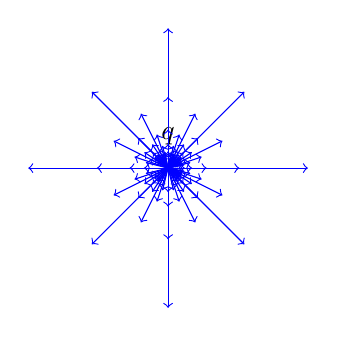
\begin{tikzpicture}[scale=.05]
  \def\q{1}
  \def\xq{0}
  \def\yq{0}
  \def\l{1}
  \def\nx{10}
  \def\ny{10}
  \draw[fill=red] (\xq,\yq) circle (0.1) node[above=5pt] {$q$};
  \foreach \i in {1,...,\nx}{
    \foreach \j in {1,...,\ny}{
      \pgfmathsetmacro{\x}{\l*(\i-\nx/2)/\nx+\xq}
      \pgfmathsetmacro{\y}{\l*(\j-\ny/2)/\ny+\yq}
      \pgfmathsetmacro{\r}{sqrt((\x-\xq)^2 + (\y-\yq)^2 + 0.01)}
      \pgfmathsetmacro{\f}{\q/(\r*\r)}
      \pgfmathsetmacro{\fx}{\f*(\x-\xq)/\r}
      \pgfmathsetmacro{\fy}{\f*(\y-\yq)/\r}
      \draw[->, blue] (\x,\y) -- ({\x+\fx},{\y+\fy});
    }
  }
\end{tikzpicture}
\end{center}


\textbf{Elektrisches Feld}

Das elektrische Feld $\mathbf{E}$ wird definiert als Kraft pro Ladung:

\begin{equation}
\mathbf{E} = \frac{\mathbf{F}}{q}
\end{equation}

wobei $\mathbf{F}$ die Kraft auf eine Ladung $q$ ist. Die Einheit des elektrischen Feldes ist Volt pro Meter (V/m).

Die Kraft $\mathbf{F}$ auf eine Ladung $q$ in einem elektrischen Feld $\mathbf{E}$ ist gegeben durch:

\begin{equation}
\mathbf{F} = q\mathbf{E}
\end{equation}

\textbf{Punktladungen im elektrischen Feld}

Für eine Punktladung $Q$ im Abstand $r$ von einem Punkt $P$ im Raum ist die Stärke des elektrischen Feldes gegeben durch das Coulomb-Gesetz:

\begin{equation}
\mathbf{E} = \frac{1}{4\pi\epsilon_0}\frac{Q}{r^2}\hat{\mathbf{r}}
\end{equation}

wobei $\epsilon_0$ die elektrische Feldkonstante ist. Die Richtung des
elektrischen Feldes ist radial von der Punktladung weg.

Für zwei Punktladungen $Q_1$ und $Q_2$ im Abstand $r$ voneinander ist die Kraft $\mathbf{F}$, die auf $Q_2$ aufgrund des elektrischen Feldes von $Q_1$ wirkt, gegeben durch das Coulomb-Gesetz:

\begin{equation}
\mathbf{F} = \frac{1}{4\pi\epsilon_0}\frac{Q_1Q_2}{r^2}\hat{\mathbf{r}}
\end{equation}

wobei $\hat{\mathbf{r}}$ der Einheitsvektor von $Q_1$ nach $Q_2$ ist.

\textbf{Feldlinien}

Feldlinien sind eine anschauliche Darstellung des elektrischen Feldes. Sie sind
so gezeichnet, dass sie immer senkrecht zu den Äquipotentialflächen stehen. Die
Dichte der Feldlinien gibt die Stärke des elektrischen Feldes an einem
bestimmten Punkt an. Die Anzahl der Feldlinien, die von einer Ladung $Q$
ausgehen, ist proportional zur Stärke der Ladung $Q$. Feldlinien beginnen immer
an positiven Ladungen und enden an negativen Ladungen oder im Unendlichen.


\end{document}
